% -*-latex-*-
%
%  The contents of this file are subject to the University of Utah Public
%  License (the "License"); you may not use this file except in compliance
%  with the License.
%
%  Software distributed under the License is distributed on an "AS IS"
%  basis, WITHOUT WARRANTY OF ANY KIND, either express or implied. See the
%  License for the specific language governing rights and limitations under
%  the License.
%
%  The Original Source Code is SCIRun, released March 12, 2001.
%
%  The Original Source Code was developed by the University of Utah.
%  Portions created by UNIVERSITY are Copyright (C) 2001, 1994
%  University of Utah. All Rights Reserved.
%

% network.tex
%

\chapter{Working with Networks}
\label{ch:workwithnets}

This section describes how to create, save, load, execute, and edit
networks.

When started with no arguments, the \command{scirun} command creates a
main window with a blank NetEdit frame. The user can create and
connect modules to form a network.


\section{Creating a Module}
\label{sec:creatingmodules}

To create a module, select its name from one of the package (\eg{} \sr)
menus' category sub-menus. Access the package menus from the
main window's menu bar and from the NetEdit frame's pop-up menu. 
 Activate The NetEdit frame's pop-up menu by clicking mouse button
3 while the mouse pointer is in the NetEdit frame (but not over a
module or connection).  The pop-up menu contains a list of category
sub-menus from the \sr{} package and other installed packages. 
Each category sub-menu provides access to the modules within the
category.

After creating a module, its graphic representation is 
placed in the NetEdit frame.

\section{Anatomy of a Module}
\label{sec:modanatomy}

%begin{latexonly}
  \newcommand{\modgraphic}%
  {\centerline{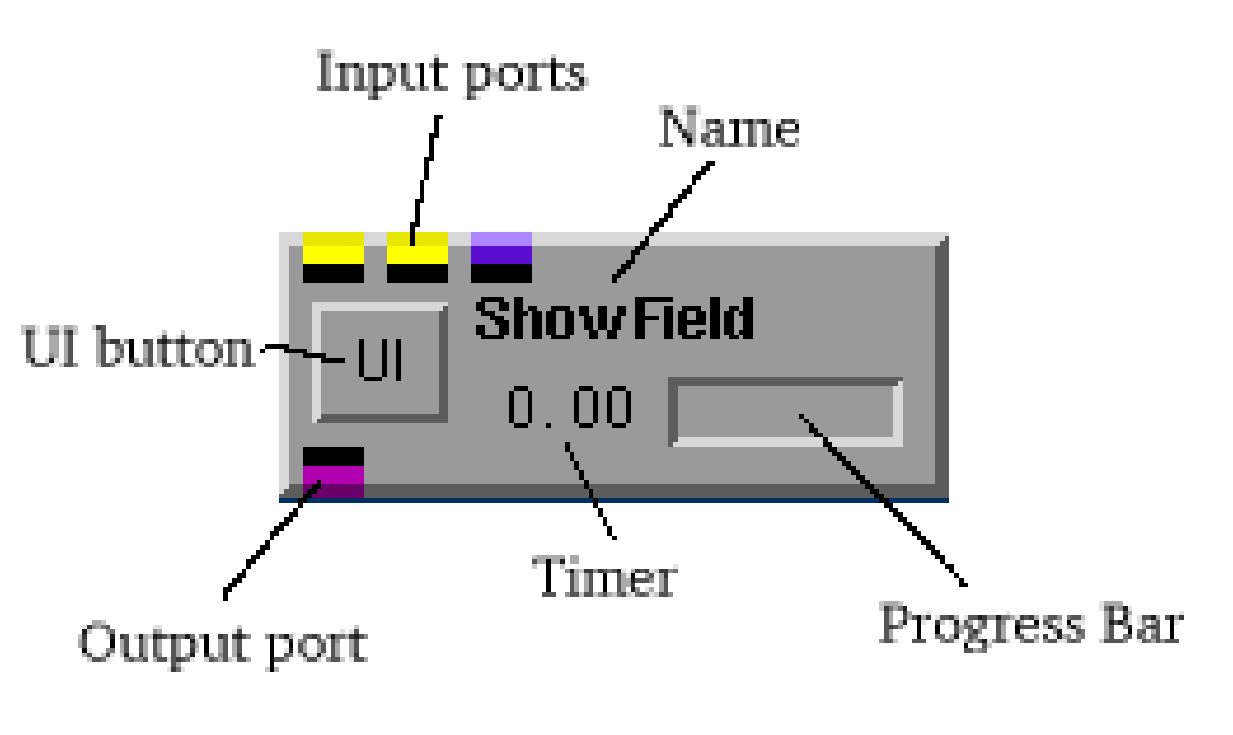
\epsfig{file=Figures/modgraphic-1.eps.gz,width=4in,
        bbllx=0, bblly=0, bburx=325, bbury=157}}}
%end{latexonly}
\begin{htmlonly}
  \newcommand{\modgraphic}{%
  \htmladdimg[align=top,width="256",alt="SCIRun Module Graphic"]
  {../Figures/modgraphic-1.gif}}
\end{htmlonly}

All modules are similarly represented by a graphic within the NetEdit frame
(see Figure~\ref{fig:modgraphic}). This graphical ``front end'' is the same
for all modules and consists of the following elements:

\begin{figure}[htb]
  \begin{makeimage}
  \end{makeimage}
  \modgraphic
  \caption{\label{fig:modgraphic} Module Graphic (\module{Show
      Field} Module)}
\end{figure}

\begin{description}
  \descitem{Module Name} The module's name.
  
  \descitem{Input Ports} Zero or more input ports located on the top
  of the module.  Each port corresponds to a data type and each data
  type has a unique color.  Table~\ref{tab:portcolors} maps port
  colors to data types.  Input ports connect to other modules' output
  ports.  Connections can only be made between ports of the same type.

  \begin{table}[htbp]
    \begin{center}
      \begin{tabular}{|l|l|}
        \hline
        \textbf{Data Type} & \textbf{Port Color} \\
        \hline
        Field & Yellow \\
        Field Set & Green \\
        Matrices & Blue \\
        Geometric Objects & Pink \\
        Color Maps & Purple \\
        Camera Path & Brown \\
        \hline
      \end{tabular}
      \caption{Data Types and their Port Colors}
      \label{tab:portcolors}
    \end{center}
  \end{table}
  
  \descitem{Output ports} Zero or more output ports located on the
  bottom of the module.  Output ports connect to other modules' input
  ports.  Every module has  at least one input or one output
  port.
  
  \descitem{UI button} Pressing the \button{UI} button displays the
  module's control dialog. Some modules have no dialog. Some have
  simple dialogs and some have complex dialogs that allow
  elaborate control over the module.  Figure~\ref{fig:moddialog} shows
  the control dialog for \module{Show Field} module.
  
  \descitem{Progress bar} Shows the module's progress.  As the module
  works toward completion of its task, the progress bar is filled
  with red, then yellow, then green.  When the Progress bar
  is green, the module is done.
  
  \descitem{Timer} Displays the amount of CPU time the module has
  consumed.  Located to the left of the progress bar.
  
  \descitem{Message Indicator} Shows the presence of messages in a
  module's log.  Colors represent message types.  Blue represents
  ``remarks'' (informational messages) and yellow represents ``warnings''
  (your attention is needed).  Click the indicator to display the
  module's log.

\descitem{Pop-up Menu} Pressing mouse button three while the mouse
  pointer is over a module gives access to the module's pop-up menu.  The
  pop-up menu gives access to the following items:
  \begin{description}
    \menuitemdesc{::Package\_Category\_Name\_Instance} This item is a
    label (not a selectable item).  It provides the module's name and
    the category and package to which the module belongs. 
    ``Instance'' is a unique number that distinguishes multiple
    instances of the same module.

    \menuitemdesc{Execute} Tells the module to
    execute (or re-execute).  This may cause other modules in the
    network to execute or``fire''
    (see \secref{Executing a Network}{sec:executenet}).

    \menuitemdesc{Help} Displays the module's help window.
    
    \menuitemdesc{Notes} Displays the module's note pad.
    The user can use the note pad to document the purpose of the module in
    the current network.

    \menuitemdesc{Destroy} Destroys the module (see \secref{Destroying
    Module(s)}{sec:destroymod}).
    
    \menuitemdesc{Show Log} Displays the module's message log.  Most
    modules write messages to their log during the course of
    their execution (see \secref{Viewing a Module's Log}{sec:viewmodslog}).
    
    \menuitemdesc{Show Status} This item is a toggle button which
    turns off/on the display of the progress indicator.  Turning off
    the progress indicator speeds up the execution of complex
    networks.
  \end{description}
\end{description}

section{Setting Module Properties}
\label{sec:setmodprops}

%begin{latexonly}
  \newcommand{\moddialog}%
  {\centerline{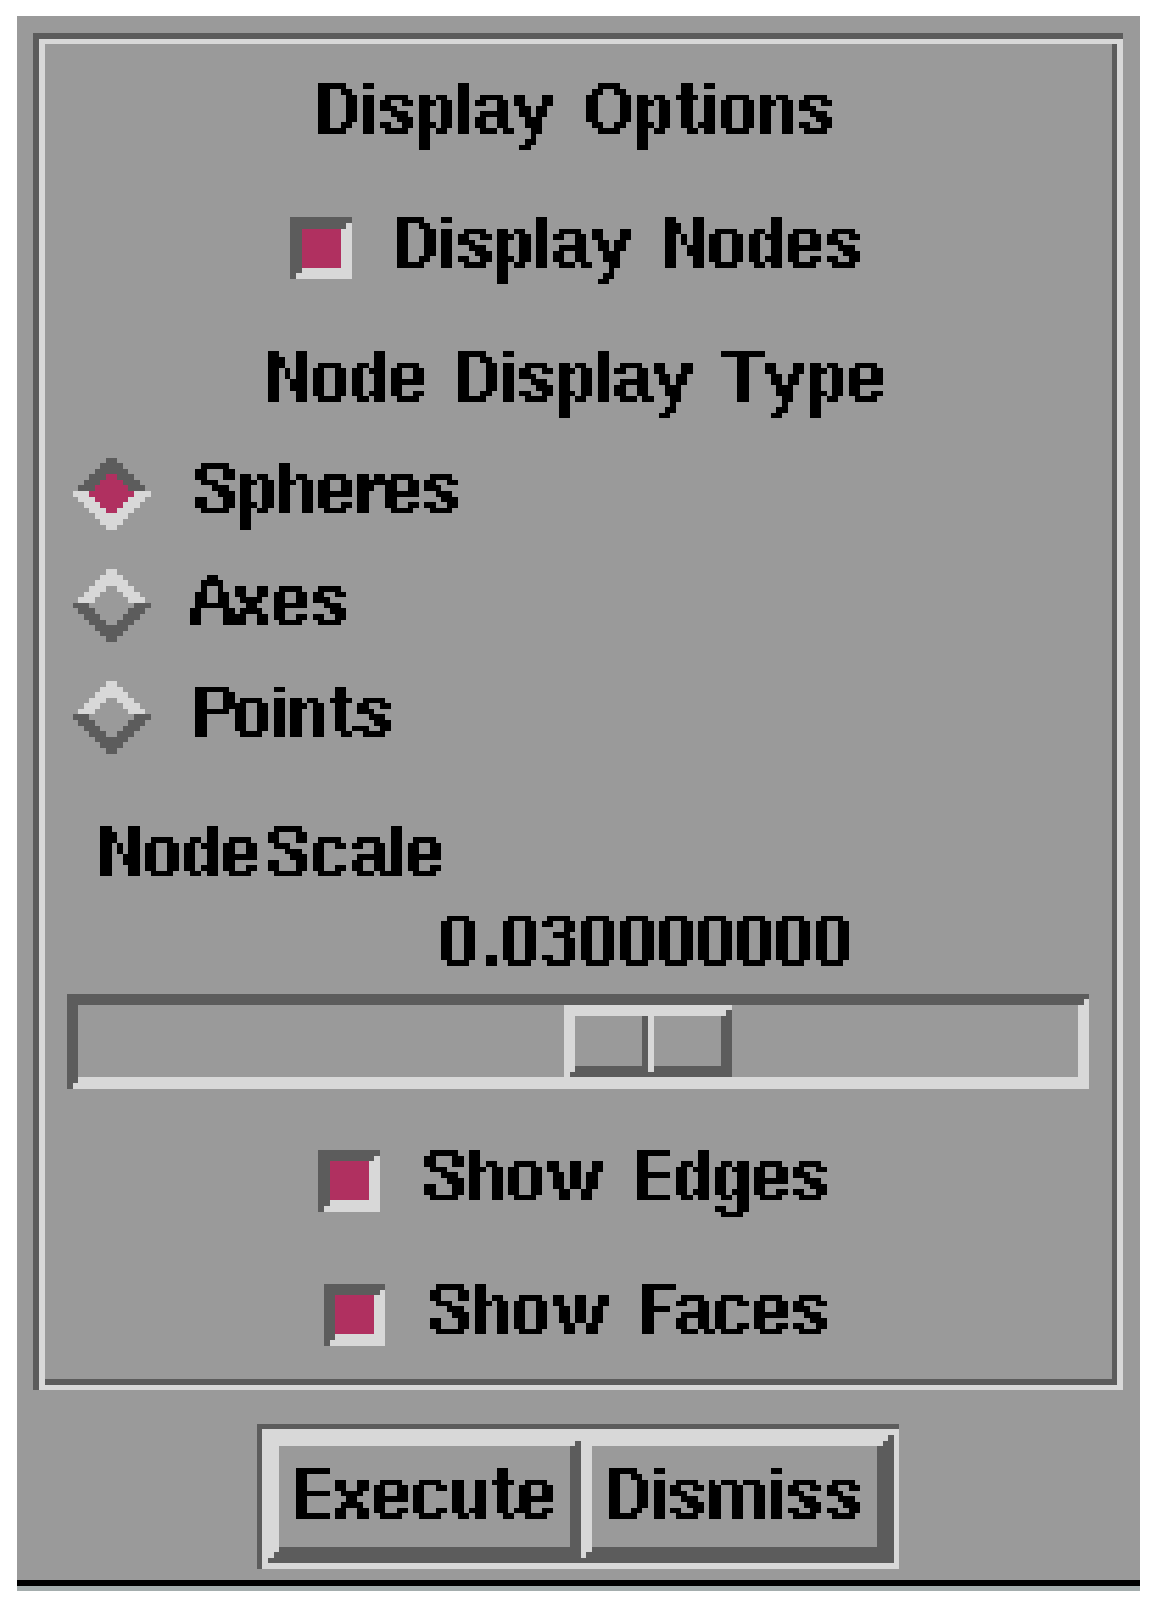
\epsfig{file=Figures/moddialog.eps.gz,
        bbllx=0, bblly=0, bburx=272, bbury=406}}}
%end{latexonly}
\begin{htmlonly}
  \newcommand{\moddialog}{%
  \htmladdimg[align=top,alt="SCIRun Module Dialog"]
  {../Figures/moddialog.gif}}
\end{htmlonly}

To change a module's properties click its \button{UI} button.  This 
displays the module's control dialog.  Use the dialog to change the
module's properties.  Each module's reference documentation explains the
use of its control dialog.  Figure~\ref{fig:moddialog} shows the control
dialog for the \module{Show Field} module.

\begin{figure}[htb]
  \begin{makeimage}
  \end{makeimage}
  \moddialog
  \caption{\label{fig:moddialog} Module \module{Show Field}'s Control Dialog
    (User Interface).}
\end{figure}

\section{Selecting Modules}
\label{sec:selectmods}

A few operations act on a group of
modules (see \secref{Moving Module(s)}{sec:movemod} and
\secref{Destroying Module(s)}{sec:destroymod}).  A group of modules
can be created in two ways:

\begin{enumerate}
\item Press mouse button two while the pointer is in the NetEdit frame,
  but not over a module or a connection.  Then drag the mouse.  This
  will draw a box outline.  Modules intersecting the box will be part
  of the group.  Release button two to complete the selection.
\item Select the first module by clicking mouse button two while the
  pointer is over a module.  Then add modules to the group by pressing
  and holding down the \keyboard{control} key while clicking on
  modules with button two.
\end{enumerate}

Selected modules will be drawn in a darker shade of grey.

Users can mix selection methods and  add modules to the group by
pressing the control key while making selections using the above methods.
If  the control key is not pressed, the previous group will be
forgotten and a new group will be created.

\section{Moving Module(s)}
\label{sec:movemod}

Modules can be moved in the NetEdit frame.  To move a module,
press mouse button one while the pointer is over a module and drag the
module to its new location.

Multiple modules can be moved at one time
(see \secref{Selecting Modules}{sec:movemod}).
Select one or more modules, then press mouse button one while the pointer is
over any one of the modules in the selected group,
and drag the modules to their new location.

\section{Destroying Module(s)}
\label{sec:destroymod}

Delete a module by selecting the \menuitem{Destroy} menu item from the
module's pop-up menu.

Multiple modules can be deleted at one time (see \secref{Selecting
  Modules}{sec:movemod}).  Select one or more modules, then choose
\menuitem{Destroy Selected} from the module's pop-up menu.

\section{Documenting a Module's Use}
\label{sec:docmodule}

It is useful to document the purpose of a module within a network.
Each module maintains a note pad for this purpose. Select
\menuitem{Notes} from the module's pop-up menu to display the module's
note pad editor.The editor allows the user to write notes on the use
of the module within the context of its network.


\section{Annotating a Module}
\label{sec:annomodule}



\section{Viewing a Module's Log}
\label{sec:viewmodslog}

Each module supports a message log.  The module writes error messages
or other types of messages to its log.  To view this log, select the
\menuitem{Show Log} item from the module's pop-up menu.

\section{Creating a Macro Module}
\label{sec:macromods}

Select more than one module using Module Selection. Right click
anywhere in the canvas. Select \menuitem{Create Macro Module}. 

\section{Setting Macro Module Properties}

The UI button opens all UIs opened when a Macro Module was created. The
menu has an option to ``Microify'', undoing the Macro Module. The
Macro Module is saved in network file.

\section{Module Blocking}
\label{sec:modblocking}

Module blocking is port blocking in code. All modules blocked together
become a `` blocked module block''. Unblocking one module unblocks all
modules in `` blocked module block''. There is an option to turn blocked
module block into Macro Module.

\section{Creating a Connection}
\label{sec:connectmods}

Mouse button two (the middle mouse button) is used to connect the output
(input) port of one module to the input (output) port of another
module. Right clicking on a connection gives access to a pop-up
menu. Use the pop-up menu to disable, delete, or annotate a connection.

To make a connection, position the mouse pointer over a module's input
(output) port.  Then press button two and drag the mouse pointer towards
another module's output (input) port.

When button two is pressed, the program shows all valid connections as
black lines.  It also draws one red colored connection, which is the
connection made if  the drag is stopped by releasing 
button two.

Make the connection by releasing button two when the pointer is over
the desired destination port or when the red colored connection is the
desired connection.  The connection is drawn using the color
corresponding to the connection's data type.

Users can connect a module's output port to the input ports of one or more
modules by repeating the procedure just described.

\section{Accessing a Connection's Pop-up Menu}
\label{sec:connectionmenu}

\section{Annotating a Connection}
\label{sec:annotatemods}

To annotate a connection, right click on a connection to bring up the pop-up 
menu and select \menuitem{Edit Annotaion}. Edit the text as any annotation.

\section{Disabling a Connection}
\label{sec:disablemods}

To disable a connection, right click on connection to bring up pop-up
menu and select disable.The connection will appear grey and no data
will pass through.

\section{Undoing a Connection}
\label{sec:undomod}

Undo only on connection deletion/addition. Undo is infinite. Undo
saves per session only, not in network

\section{Deleting a Connection}
\label{sec:deleteconnections}

Delete a connection by pressing mouse button three while the pointer is
over a connection.

\section{Executing a Network}
\label{sec:executenet}

``Network Execution'' means one or more modules must be executed in a
coordinated fashion. 
\sr{}'s \dfn{scheduler} manages the coordinated execution of modules.

Note that some modules need to be compiled before they are
executed (see \secref{Dynamic Compilation}{sec:dyncomp}).  Compilation
delays execution of the network.  This delay occurs only one time
(per module).  After a module is compiled, it does not need to be
compiled again.  Modules change color during compilation.

\subsection{The Basics}

The scheduler is invoked when an event \dfn{triggers} a
module's execution.  The scheduler creates a list of all modules that
must execute in coordination with the triggered module. Modules
\dfn{upstream} (directly or indirectly) from the triggered module are 
put on the execution list if they have not previously executed.
All modules \dfn{downstream} from the triggered module are put
on the execution list.  Once the scheduler determines which modules must be
executed, it executes them (in parallel where possible).

Network execution is mostly transparent.  That is, events that trigger
module execution usually generate automatically. Sometimes,
however, the user must manually
generate a triggering event by choosing the \menuitem{Execute} item from a
module's pop-up menu.

\subsection{Details}

Each module executes in its own thread and blocks (waits) until its
upstream modules can supply it with data.  After a module completes
its computation, it sends the results to its downstream modules.  This
completes a module's execution cycle.  The module will not have
another chance to receive data from its input ports and send data to
its output ports until some event puts the module back on the
scheduler's execution list.

This behavior prevents modules from computing in an iterative fashion,
sending intermediate results to their downstream modules, because
downstream modules cannot receive results until they are in their
execution cycle. Downstream modules would need to be executed each time the
upstream module posts an intermediate result.


\subsection{Intermediate Results}

Some modules are designed to be used in an iterative fashion.  They send
data to their output ports in a special way.  They use a method called
\icode{send\_intermediate} to send the results of each iteration.  When
this method is used, the scheduler (re)executes downstream modules each time
the upstream module posts its next result.  Downstream modules are
able to receive the results of each iteration as soon as the
upstream module sends them.

Modules \module{SolveMatrix} and \module{MatrixSelectVector} (from the
\package{\sr} package and \category{Math} category) are examples of modules
that compute iteratively using the \icode{send\_intermediate} method.

\subsection{Feedback Loops}

Some modules are designed to be used exclusively in feedback
loops. Their output ports can be connected
directly or indirectly to their input ports.  These modules also use the
\icode{send\_intermediate} method.

Examples of feedback modules are \module{DipoleSearch} and
\module{ConductivitySearch} from the \category{Inverse} category of the
\package{BioPSE} package and \module{BuildElemLeadField} from the
\category{LeadField} category of the \package{BioPSE} package.

\section{Documenting a Network}
\label{sec:docnetwork}

It is useful to document the function of a network.  A network's note
pad is used for this purpose.  To edit the network's note pad,
select the \menuitem{Add Info} item from the main window's \menu{File}
menu.  This will display the network's note pad editor.  The editor
allows the user to write notes on the purpose and use of the network.

\section{Saving a Network}
\label{sec:savenet}

\sr{} can save networks to files.  Network files have an extension of
\filename{.net} (in the past they also had .sr and .uin
extensions).  

To save a network, select \menuitem{Save} item from the main window's
\menu{File} menu.  A file browser dialog will prompts for the
name and location of the network file.

If  changes are made to an existing network,  \menuitem{Save} 
saves changes made to an existing net file.

Save an existing network under a new name using the
\menuitem{Save As...} menu item.  A file browser dialog prompts
for the new name of the network file.  Subsequent uses of
\menuitem{Save} saves changes to the newly created file.

Network files are  \dfna{Tool Command Language}{TCL} scripts.
These files can be edited, however the reasons for doing so are beyond
the scope of this guide.

\section{Loading a Network}
\label{sec:opennet}

To load a network file, select the \menuitem{Load} item from the main
window's \menu{File} menu.   A file browser dialog will prompt for the
name and location of the network file.

Note that loading a network file adds the network to an existing network in
the NetEdit frame, possibly overlapping the networks.

\section{Inserting a Network}
\label{sec:insertnetwork}

To avoid merging networks, select the
\menuitem{Insert} item from the main window's \menu{File} menu. This
option allows the user to place one \sr{} network next to another,
avoiding overlap.  A file browser dialog prompts the user for the name and
location of the network file.

The new network is inserted into the upper left corner of the
NetEdit frame.  If a network of modules already exists in the NetEdit
frame, the \menuitem{Insert} command places a new network to the
immediate right of the existing network.

\section{Clearing a Network}
\label{sec:clearnetwork}

To remove all modules and connections from the 
NetEdit frame, select the \menuitem{Clear} item from the main window's
\menu{File} menu in order.  A text box appears, confirming whether the
user wants to proceed with or cancel the clearing operation.

\section{Navigating a Network}
\label{sec:navnetwork}

A complex network may not be entirely visible in the NetEdit frame.
Use the NetEdit frame's scroll bars or the network view tool to view
complex networks.

The Global View Frame shows the entire ``network world.''  The small
rectangular region (outlined in black) in the Global View Frame is the
network view tool and a window on the network world. The
position of the view tool determines the part of the network 
visible in the NetEdit frame.  To view other parts of the network, press
button one while the pointer is anywhere in the Global View Frame -- this 
moves the tool to the location of the pointer --  then drag the tool to the
new location.


\section{The \sr{} Shell}
\label{sec:termapp}

After starting, \sr{} runs a shell-like application in the terminal
window. This shell displays the prompt
\screen{scirun\ra} in the terminal window.  This program is a
\dfna{Tool Command Language}{TCL} shell program that has been extended with
\sr{} specific commands.

It is possible to type \tcl{} \sr{} commands at the prompt.  For
instance, to load a network type \keyboard{source
  \ptext{network file name}}.  This has the same effect as the \menu{File}
menu's \menuitem{Load} command.

%\incomplete{}


%%% Local Variables: 
%%% mode: latex
%%% TeX-master: t
%%% End: 
